\documentclass[customlatinfont=gyre,displaycommittee=false,blankpage=false]{template/hkust-thesis-v0.11.6/hkustthesis}
\hkustsetup{info={degree={phd},title={Structural Augmented Reasoning for Language Models},keywords={knowledge graphs,language models,retrieval},author={Yubo Wang},school={School of Engineering},department={Department of Computer Science and Engineering},program={Computer Science and Engineering},major={},supervisor={[Supervisor name pending author confirmation]},co-supervisor={},submit-month={[Submission month pending]},submit-date={[Signature date pending]},defend-date={},depthead={[Head name and title pending confirmation]},reviewer={},reviewerdept={},reviewerext={},city={Hong Kong}}}
\addbibresource{template/template-smoke.bib}
\newtheorem{smokecondition}{Condition}[chapter]
\begin{document}
\frontmatter
\maketitle
\begin{abstract}
This document tests the typesetting of an English PhD thesis on structural augmentation for language models. It contains one published MGRAG overview figure, the published dataset statistics, a mathematical expression for selective KV recomputation, and a concise algorithmic description of its retrieval workflow. The research content is included to test figure clarity, table width, mathematical fonts, algorithm formatting, bibliography integration, and page numbering. Author-specific signature information remains explicitly marked for confirmation. This is a template evaluation document rather than a submission copy or a research chapter.
\end{abstract}
\authorization
\signaturepage
\begin{acknowledgements}
Acknowledgments will be supplied by the author. This page tests the position and layout of the acknowledgments environment.
\end{acknowledgements}
\tableofcontents
\listoffigures
\listoftables
\mainmatter
\chapter{Semantic Graph Matching for Multimodal Evidence}
\label{ch:smoke}
\section{Query-aware Retrieval}
This section is based on the published MGRAG paper~\cite{smoke:mgrag}. MGRAG ranks multimodal evidence, builds a query-specific graph incrementally, and matches paths in a query graph to semantically corresponding evidence subgraphs. Its retrieval pipeline uses the captions of images for coarse-grained ranking with a text encoder. Text documents are split into overlapping chunks. The ranked text and image evidence then provide the input for query-aware graph construction.

Graph construction proceeds through the ranked chunks until a semantic match is found or an iteration limit is reached. A query path can correspond to several facts in the evidence graph, so matching operates on semantic representations of paths and subgraphs. The generator receives the matched graph sequence, the multimodal chunks used during graph construction, and the query. Figure~\ref{fig:smoke:overview} reproduces the original overview without changing any graphical elements.

\begin{figure}[tbp]
\centering
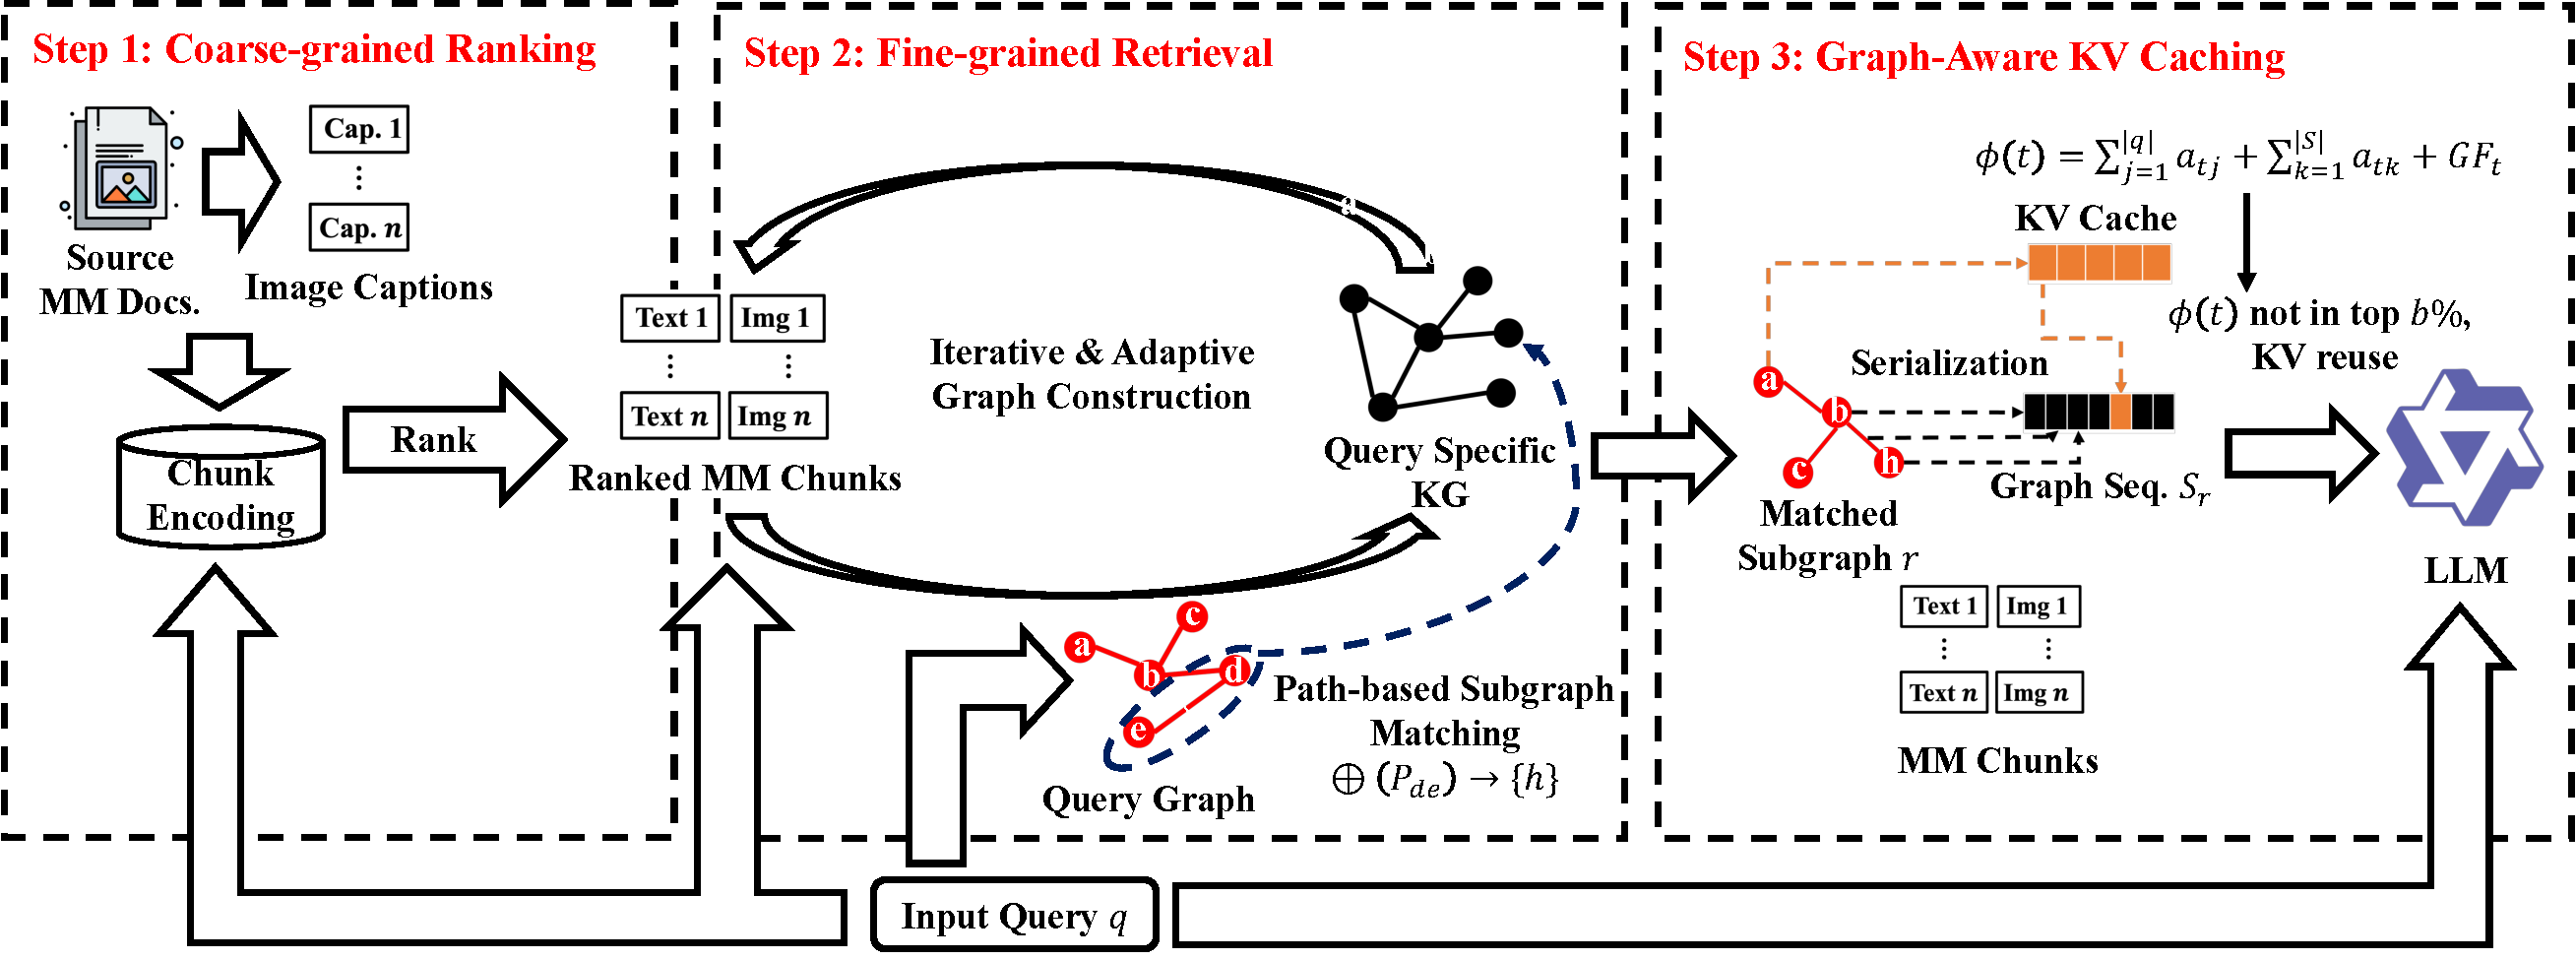
\includegraphics[width=\textwidth]{template/assets/pipeline_new.pdf}
\caption{MGRAG overview, reproduced from Figure 2 of the published paper~\cite{smoke:mgrag}, p.\ 2484. The stages rank chunks, construct and match a query-specific graph, and selectively recompute KV states.}
\label{fig:smoke:overview}
\end{figure}

\section{Graph-aware Context Computation}
MGRAG scores tokens using attention to the query, attention to the serialized graph, and graph features. With the source paper's notation, its token recomputation score is
\begin{equation}
\label{eq:smoke:score}
\phi(t)=\sum_{j=1}^{|q|}a_{tj}+\sum_{k=1}^{|S_r|}a_{tk}+GF_t^q.
\end{equation}
At each transformer layer, the tokens with scores in the highest $b\%$ are recomputed. The remaining KV states are reused. Equation~\ref{eq:smoke:score} is the MGRAG row of published Table 2 (p.\ 2483); it is included here to test mathematical typography and references. The score combines local attention information with degree, betweenness, closeness, and eigenvector centrality features of associated graph facts. These operations concern selective recomputation during answer generation.

\begin{algorithm}[tbp]
\caption{MGRAG retrieval workflow from the published overview}
\label{alg:smoke:workflow}
\begin{algorithmic}[1]
\REQUIRE Query $q$, ranked multimodal chunks, iteration limit $\mu$
\STATE Construct the query graph from $q$
\FOR{each ranked chunk, up to $\mu$ iterations}
\STATE Extract query-related entities and relations from the chunk
\STATE Enrich the query-specific evidence graph
\STATE Search for a path-based semantic match
\IF{a matched evidence subgraph is found}
\STATE Stop graph construction
\ENDIF
\ENDFOR
\STATE Serialize the matched evidence subgraph for answer generation
\end{algorithmic}
\end{algorithm}

\section{Evaluation Inputs}
Table~\ref{tab:smoke:datasets} reproduces every cell of the dataset statistics in published Table 3 (p.\ 2488). The experiment uses MMQA and six MRAMG subsets. The caption in the publication refers to ``7 sub dataset of the MRAMG benchmark'', while the actual columns and the dataset paragraph identify six MRAMG subsets and MMQA. The column values are preserved below, and this caption discrepancy is recorded in the template evaluation notes rather than resolved through an invented dataset.

\begin{table}[tbp]
\centering
\caption{Published MGRAG dataset statistics. T and I denote textual and image query modalities. Numerical values and abbreviations reproduce Table 3 of the published paper~\cite{smoke:mgrag}.}
\label{tab:smoke:datasets}
\small
\setlength{\tabcolsep}{3pt}
\begin{tabular}{lrrrrrrr}
\toprule
Statistic & MMQA & Wiki & Wit & Recipe & Arxiv & Manual & Web\\
\midrule
Query Modality & T / I & T & T & T & T & T & T\\
Queries & 951 & 500 & 600 & 2,360 & 200 & 390 & 750\\
Texts & 218,285 & 538 & 639 & 1,528 & 101 & 40 & 1,500\\
Images & 57,058 & 538 & 639 & 8,569 & 337 & 2,607 & 1,500\\
Corpus Size & 22.5M & 680k & 478k & 1.1M & 136k & 420k & 215k\\
Query Hops & 1--2 & 2--5 & 2--4 & 1--6 & 3--4 & 2--6 & 2--3\\
Avg Query Hops & 1.5 & 3.0 & 2.8 & 3.3 & 3.1 & 3.7 & 2.4\\
\bottomrule
\end{tabular}
\end{table}

The dataset statistics distinguish the size of the source corpus from the number of evaluation queries. MMQA provides 951 queries over 218,285 text records and 57,058 images. The MRAMG subsets differ in domain, corpus size, and query-hop distribution. These settings define the reported evaluation inputs; they are not pooled into a new aggregate benchmark in this document. The table is included to test a wide eight-column table with mixed numerical and textual entries.

\begin{smokecondition}
A mathematical statement can be numbered and cross-referenced independently of equations and algorithms.
\end{smokecondition}
This typesetting-only statement verifies the theorem environment. It asserts no new algorithmic result.
\printbibliography[heading=bibintoc,title=References]
\appendix
\chapter{Template Verification Notes}
The title page is counted as Roman page i and currently displays that number, matching the visible title-page sample. The official sample's body guidance also says that i is not displayed on the title page. Final display requires confirmation from the submission office. All draft placeholders in the front matter must be replaced with author-confirmed information before submission.
\end{document}
